\documentclass[11pt,a4paper]{report}%especifica o tipo de documento que tenciona escrever: carta, artigo, relatório... neste caso é um relatório
% [11pt,a4paper] Define o tamanho principal das letras do documento. caso não especifique uma delas, é assumido 10pt
% a4paper -- Define o tamanho do papel.
\usepackage{float}
\usepackage[portuges]{babel}%Babel -- irá activar automaticamente as regras apropriadas de hifenização para a língua todo o
                                   %-- o texto gerado é automaticamente traduzido para Português.
                                   %  Por exemplo, “chapter” irá passar a “capítulo”, “table of contents” a “conteúdo”.
                                   % portuges -- específica para o Português.
\usepackage[utf8]{inputenc} % define o encoding usado texto fonte (input)--usual "utf8" ou "latin1

\usepackage{graphicx} %permite incluir graficos, tabelas, figuras
\usepackage{url} % para utilizar o comando \url{}
\usepackage{enumerate} %permite escolher, nas listas enumeradas, se os iems sao marcados com letras ou numeros-romanos em vez de numeracao normal

%\usepackage{apalike} % gerar biliografia no estilo 'named' (apalike)

\usepackage{color} % Para escrever em cores

\usepackage{multirow} %tabelas com multilinhas
\usepackage{array} %formatação especial de tabelas em array

\usepackage[pdftex]{hyperref} % transformar as referências internas do seu documento em hiper-ligações.

%Exemplos de fontes -- nao e vulgar mudar o tipo de fonte
%\usepackage{tgbonum} % Fonte de letra: TEX Gyre Bonum
%\usepackage{lmodern} % Fonte de letra: Latin Modern Sans Serif
%\usepackage{helvet}  % Fonte de letra: Helvetica
%\usepackage{charter} % Fonte de letra:Charter

\definecolor{saddlebrown}{rgb}{0.55, 0.27, 0.07} % para definir uma nova cor, neste caso 'saddlebrown'

\usepackage{listings}  % para utilizar blocos de texto verbatim no estilo 'listings'
%paramerização mais vulgar dos blocos LISTING - GENERAL
\lstset{
	basicstyle=\small, %o tamanho das fontes que são usadas para o código
	numbers=left, % onde colocar a numeração da linha
	numberstyle=\tiny, %o tamanho das fontes que são usadas para a numeração da linha
	numbersep=5pt, %distancia entre a numeração da linha e o codigo
	breaklines=true, %define quebra automática de linha
    frame=tB,  % caixa a volta do codigo
	mathescape=true, %habilita o modo matemático
	escapeinside={(*@}{@*)} % se escrever isto  aceita tudo o que esta dentro das marcas e nao altera
}
%
%\lstset{ %
%	language=Java,							% choose the language of the code
%	basicstyle=\ttfamily\footnotesize,		% the size of the fonts that are used for the code
%	keywordstyle=\bfseries,					% set the keyword style
%	%numbers=left,							% where to put the line-numbers
%	numberstyle=\scriptsize,				% the size of the fonts that are used for the line-numbers
%	stepnumber=2,							% the step between two line-numbers. If it's 1 each line
%											% will be numbered
%	numbersep=5pt,							% how far the line-numbers are from the code
%	backgroundcolor=\color{white},			% choose the background color. You must add \usepackage{color}
%	showspaces=false,						% show spaces adding particular underscores
%	showstringspaces=false,					% underline spaces within strings
%	showtabs=false,							% show tabs within strings adding particular underscores
%	frame=none,								% adds a frame around the code
%	%abovecaptionskip=-.8em,
%	%belowcaptionskip=.7em,
%	tabsize=2,								% sets default tabsize to 2 spaces
%	captionpos=b,							% sets the caption-position to bottom
%	breaklines=true,						% sets automatic line breaking
%	breakatwhitespace=false,				% sets if automatic breaks should only happen at whitespace
%	title=\lstname,							% show the filename of files included with \lstinputlisting;
%											% also try caption instead of title
%	escapeinside={\%*}{*)},					% if you want to add a comment within your code
%	morekeywords={*,...}					% if you want to add more keywords to the set
%}

\usepackage{xspace} % deteta se a seguir a palavra tem uma palavra ou um sinal de pontuaçao se tiver uma palavra da espaço, se for um sinal de pontuaçao nao da espaço

\parindent=0pt %espaço a deixar para fazer a  indentação da primeira linha após um parágrafo
\parskip=2pt % espaço entre o parágrafo e o texto anterior

\setlength{\oddsidemargin}{-1cm} %espaço entre o texto e a margem
\setlength{\textwidth}{18cm} %Comprimento do texto na pagina
\setlength{\headsep}{-1cm} %espaço entre o texto e o cabeçalho
\setlength{\textheight}{23cm} %altura do texto na pagina

% comando '\def' usado para definir abreviatura (macros)
% o primeiro argumento é o nome do novo comando e o segundo entre chavetas é o texto original, ou sequência de controle, para que expande
\def\darius{\textsf{Darius}\xspace}
\def\antlr{\texttt{AnTLR}\xspace}
\def\pe{\emph{Publicação Eletrónica}\xspace}
\def\titulo#1{\section{#1}}    %no corpo do documento usa-se na forma '\titulo{MEU TITULO}'
\def\super#1{{\em Supervisor: #1}\\ }
\def\area#1{{\em \'{A}rea: #1}\\[0.2cm]}
\def\resumo{\underline{Resumo}:\\ }

%\input{LPgeneralDefintions} %permite ler de um ficheiro de texto externo mais definições

\title{Processamento de Linguagens (3º ano de Curso)\\
       \textbf{Trabalho Prático 2}\\ Relatório de Desenvolvimento
       } %Titulo do documento
%\title{Um Exemplo de Artigo em \LaTeX}
\author{José Pereira\\ (a82880@alunos.uminho.pt) \and Ricardo Petronilho\\ (a81744@alunos.uminho.pt)
       } %autores do documento
\date{\today} %data

\begin{document} % corpo do documento
\maketitle % apresentar titulo, autor e data

\begin{abstract}  % resumo do documento
O projeto elaborado na Unidade Curricular de Processamento de Linguagens do Mestrado integrado em Engenharia Informática da Universidade do Minho, tem como principal objetivo o processamento de informação contida em ficheiros do tipo Córpora, utilizando para isso a ferramenta \emph{awk}.
\end{abstract}

\tableofcontents % Insere a tabela de indice
%\listoffigures % Insere a tabela de indice figuras
%\listoftables % Insere a tabela de indice tabelas

\chapter{Introdução} \label{chap:intro} %referência cruzada

Na unidade curricular de Processamento de Linguagens, do Mestrado integrado em Engenharia Informática da Universidade do Minho, foi nos proposta a elaboração do exerício 5, que se trata da elaboração de vários scripts que através da aplicação \emph{awk}, processa ficheiros, sendo o principal objetivo filtrar as informações mais importantes.\\\\
Deste modo, os ficheiros analisados contém extratos com as respetivas palavras e associado a estas informação de anotação frásica e morfossintática.\\\\Para a elaboração destes scripts, foi necessária uma análise dos vários ficheiros disponibilizados pela equipa docente, que contêm os extratos. 
\\\\A nível de trabalho adicional, tentou-se em todos os problemas gerar uma página \emph{HTML}, com um formato mais apelativo para leitura, do que no terminal, sendo que estes processos serão especificados mais adiante.


\chapter{Análise e Especificação} \label{chap:analiseEspecificacao} %capitulo e referencia cruzada
\section{Contextualização do problema} \label{sec:descricaoProblema} %seccao e referencia cruzada
O objetivo central deste trabalho prático é focado no processamento da informação de grandes ficheiros.\\\\Neste caso, tal como já foi referenciado anteriormente o ficheiro para processamento contém extratos e informação de anotação frásica e morfossintática associada a cada palavra contida nestes.\\\\Deste modo, utilizando a aplicação \emph{awk}, definiu-se um script capaz de contar o número de extratos contidos num ficheiro, calcular o número de ocorrências de nomes próprios, criar uma página \emph{HTML} com as listas dos verbos, substantivos, adjetivos e advérbios contidos no ficheiro e por fim criar uma página \emph{HTML} com o dicionário implicíto no córpora.


\chapter{Concepção/desenho da Resolução}

\section{API}
Com uma análise geral aos vários problemas, entendeu-se de imediato que existem várias funções que serão utilizadas nos diferentes problemas. \\\\Deste modo decidiu-se criar um ficheiro denominado \emph{api.awk} que inclui as funções da API, das quais: \textbf{beginHTML()}, que cria o ficheiro \emph{index.html} e a estrutura inicial desse mesmo ficheiro, \textbf{endHTML()}, que faz o inverso, ou seja, estrutura o fim do ficheiro \emph{HTML}, \textbf{link()}, gera o código necessária \emph{HTML}, para um \emph{link} e por fim, \textbf{createHTMLdir()}, remove caso exista e cria a diretoria \textbf{html/}, para guardar os ficheiros necessaários para as páginas \emph{HTML}. 
\newpage
\section{Problema 1}
O primeiro problema pede para contar o número de extratos existentes nos ficheiros fornecidos. Desta froma foi utilizado o padrão \textbf{BEGIN} para inicialmente especificar qual o \textbf{separador de registo}, neste caso é uma linha em branco ou seja: RS = ``\textbackslash n\textbackslash n``.
\\\\
No fim imprime-se dentro do padrão \textbf{END} o número de extratos percorridos utilizando a variável \textbf{NR}. 
\newpage

\section{Problema 2}
Este problema pede para listar os nomes próprios e o número de ocorrências dos mesmos. 
\\\\
Inicialmente definiu-se dentro do padrão \textbf{BEGIN} que o \textbf{separador de registo} corresponde á mudança de linha, não interessa que seja a sepração entre extratos uma vez que para o contexto deste problema o conteúdo útil é cada palavra e a sua caracterização, assim RS = ``\textbackslash n`` e que o \textbf{separador de campos} corresponde um espaço, isto é FS = `` ``.
\\\\
Definiu-se uma \textbf{exrpessão regular} para apenas processar nomes próprios ao longo da iteração do ficheiro, sendo a mesma: \$4 \textasciitilde/NP.*/, o campo \textbf{\$4} correspondente à \textbf{TAG} da palavra.
\\\\
Existe um array denominado \textbf{counter} que aramazena para cada nome o número de ocorrências atuais do mesmo, desta forma quando se deteta um nome próprio é incrementado o número de ocorrências do mesmo: \textbf{counter[tolower(\$2)]++}, o campo \textbf{\$2} corresponde ao nome próprio. 
\\\\
É utilizada a função \textbf{tolower()} para garantir que não se conta mais que uma vez a mesma palavra, por exemplo as palavras: \textbf{"sim"} e \textbf{"Sim"} são a mesma no entanto caso não se usa-se a função \textbf{tolower()} seriam detetadas como diferentes.
\\\\
No fim dentro do padrão \textbf{END} impreme-se os resultados obtidos numa página \textbf{HTML}. Todos os ficheiros \textbf{.html} são armazenados numa pasta \textbf{html/} sendo a mesma criada através da função \textbf{createHTMLdir()}. Para imprimir o \textbf{header} e \textbf{footer} de cada página foram criadas as funções \textbf{beginHTML()} e \textbf{endHTML()} respetivamente.
\\\\
Finalmente falta imprimir a lista dos nomes próprios e o respetivo número de ocorrências à frente, para tal é percorrido o array \textbf{counter} com o critério de iteração necessário, sendo o mesmo especificado da seguinte forma: \textbf{PROCINFO[``sorted\textunderscore in``] = ``comparator``}, sendo a função \textbf{comparator()} a que estabelece o critério de ordenação, que neste caso é \textbf{descendente} do número de ocorrências.
\newpage 

\section{Problema 3}
O objetivo deste problema é calcular a lista de verbos, substantivos, adjetivos e advérbios e criar uma página \emph{HTML} com esta informação.
\\\\Deste modo, começou-se por definir os campos RS = ``\textbackslash n`` e FS = `` `` no padrão \textbf{BEGIN}, pois, as palavras no extrato estão separadas por um ``\textbackslash n`` e a informação de cada palavra por um espaço.
\\\\De seguida, determinou-se o campo necessário para a identificação do tipo de palavra (verbo, substativo, adjetivo e advérbio), que neste caso é o campo quatro (\$4), ou seja, \emph{pos-tag}.
\\\\Assim, detetou-se que as tags começam  por uma determinada letra, que identificam o tipo de palavra (V=verbo, N=substantivo, A=adjetivo e R=advérbio), ou seja, os padrões usados são:

\begin{itemize}
  \item verbos: \$4\~/V.*/
  \item substantivos: \$4\~/N.*/ 
  \item adjetivos: \$4\~/A.*/ 
  \item advérbios: \$4\~/R.*/
\end{itemize}

De seguida, definiu-se o array de duas dimensões denominado por \emph{words}, que é responsável por guardar cada tipo de palavra e o respetivo número de ocorrências, isto é, as linhas correspondem ao tipo de palavra (verbo, substantivo, adjetivo e advérbio), e as colunas correspondem às palavras desse tipo, guardando o número de ocorrências das mesmas.

\begin{center}
\begin{tabular}{ |c|c|c|c| } 
 \hline
"verbos"  & "ser" & "ter" & ...\\ 
          & 1170 & 1106 & ...\\
 \hline
 "substantivos"& "harry" & "que" & ... \\
               & 1430 & 1369 & ...\\
 \hline
 "adjetivos"& "grande" & "enorme" & ...\\
            & 114 & 96 & ...\\
 \hline
"adverbios" & "que" & "mais" & ...\\
            & 1353 & 337 & ...\\ 
 \hline
\end{tabular}
\caption{\label{tab:table-name}\\Tabela representativa do array \emph{words}.}
\end{center}

Atente-se que o motivo de se armazenar o lema e não a palavra é para que, por exemplo as palavras \textbf{"disseste"} e \textbf{"disse"} sejam contabilizadas como o mesmo verbo \textbf{"dizer"}.\\

\\Deste modo, aos padrões referidos anteriormente, associa-se o array do respetivo tipo de palavra, ou seja, por exemplo, tal como se pode verificar no código abaixo, para o padrão que captura verbos, vai-se ao array que está na linha correspondente a "verbos" e à coluna correspondente ao lema da palavra encontrada (\$3) e incrementa-se uma unidade, que no final será usada para fins estatísticos.
\\\\A razão pela qual se usa o \emph{tolower}, tal como já foi referido anteriormente, é para não haver repetições da mesma palavra, nos casos onde a diferença é na letra inicial ser maíuscula ou minúscula.

\begin{verbatim}
$4~/V.*/{
    words["verbos"][tolower($3)]++
}
\end{verbatim}

\\\\No padrão \textbf{END}, começa-se por chamar a função \textbf{createHTMLdir()}, que é responsável por criar a diretoria, onde são guardados todos os ficheiros necessários para a página \emph{HTML}, tal como já foi referênciado no problema anterior.
\\\\De seguida, chama-se a função principal deste script, denominada por \textbf{listing()}, que é responsável por listar os diferentes tipos de palavras em diferentes páginas, onde, as palavras são ordenadas pelo seu número de ocorrências. Importante referir, que logo, no ínicio desta função, é chamada para cada ficheiro a função \textbf{header()}, responsável por criar os ficheiros \textbf{.html} para cada lista e estruturar o código \emph{HTML} inicial.
\\\\Como a informação foi guardada num array bi-dimensional, torna-se fácil o processo de listar as palavras por tipos em diferentes ficheiros, pois itera-se o mesmo, por linha, escrevendo os dados para o ficheiro específico do tipo de palavra (tipoDePalavra.html), onde o nome do mesmo corresponde à linha do array. Ainda nesta função, faz-se a análise estatística, contando-se o número de ocorrências de palavras de cada tipo sendo estes valores guardados em variáveis para depois serem apresentados. \\\\Importante referir, que as palavras nos ficheiros são ordenadas pelo seu número de ocorrências, isto consegue-se, tal como já foi referenciado anteriormente, com a adição da linha \textbf{PROCINFO[``sorted\textunderscore in``] = ``comparator``} e definição da função \textbf{comparator} que é utilizada para o critério de ordenação.
\\\\Por fim, são chamadas funções responsáveis pela estrutuação dos ficheiros \emph{HTML}, das quais, \textbf{meta()}, que é responsável por criar a página \emph{index.html}, com \emph{links} a redirecionar para as páginas com as listas e a apresentação dos dados estatísticos 
\newpage


\section{Problema 4}
O propósito deste programa é determinar e apresentar o dicionário implícito nos ficheiros fornecidos. 
\\\\
Incialmente definiu-se dentro do padrão BEGIN os valores de RS = ``\textbackslash n`` e FS = `` ` uma vez que cada linha é considreada um registo e os campos dentro da linha são sperados por um espaço.
\\\\
De seguida definiu-se as 8 \textbf{expressões regulares} relvantes para determinar o dicionário:

\begin{itemize}
  \item verbos: \$4\~/V.*/
  \item nomes: \$4\~/N.*/ 
  \item adjetivos: \$4\~/A.*/ 
  \item advérbios: \$4\~/R.*/
  
  \item preposições: \$4\~/S.*/
  \item determinantes: \$4\~/D.*/
  \item conjunções: \$4\~/C.*/
  \item pronomes: \$4\~/P.*/
\end{itemize}

Sendo que o campo \textbf{\$4} corresponde à palavra detetada. Note-se que não se processou por exemplo os sinais de pontuação apesar de nos ficherios fornecidos serem descritos, uma vez que não é um elemento relevante para a descrição num dicionário.
\\\\
Posterioremente, definiu-se uma matriz denominada por \textbf{dic}, nome alusivo a \textbf{dicionário}, que para cada \textbf{lema} e \textbf{palavra} aramazena a respetiva \textbf{TAG} que descreve efetivamente a palavra. A seguinte figura representa gráficamete a informação da matriz \textbf{dic}.

\begin{center}
\begin{tabular}{ |c|c|c|c|c| } 
 \hline
"ser"  & "era" & "seja" & "sou" & ...\\ 
     & VMII1S0 & VMSP1S0 & VMIP1S0 &  ...\\
 \hline
"ter"  & "tendo" & "terei" & "tivera" & ...\\ 
     & VMG0000 & VMIF1S0 & VMIM1S0 &  ...\\
\hline
"..."  & "..." & "..." & "..." & ...\\ 
     & ... & ... & ... &  ...\\
\hline
\end{tabular}
\caption{\label{tab:table-name}\\Tabela representativa da matriz \textbf{dic}.}
\end{center}

Segundo a informação da matriz em cima, por exemplo, a palavra \textbf{``era``} tem a \textbf{TAG=VMII1S0}, por isso é um verbo \textbf{(VM)} no modo indicativo \textbf{(I)} no pretérito imperfeito \textbf{(I)} na 1ª \textbf{(1)} pessoa no singular \textbf{(S)}. No momento de armazenamento tanto do lema como das palavras, utilizou-se a função \textbf{tolower()} para não contabilizar palavras repetidas. 
\\\\
Dentro do padrão \textbf{END}, evoca-se a função \textbf{createHTMLdir()}, criando a diretoria, onde são guardados todos os ficheiros necessários para a página \emph{HTML}. 
\\\\
A variável \textbf{PROCINFO[``sorted\textunderscore in``] = ``comparator``} garante que a iteração sobre a matriz \textbf{dic} é feita por ordem alfabética. 
\\\\
Para a apresentação do dicionário utilizou-se a convenção que todos os dicionários físicos ou virtuais usam: existe uma página \emph{HTML} para cada letra do alfabeto fonético internacional (de A a Z) assim, por exemplo os \textbf{lemas}: \textbf{"comer"} e \textbf{"começar"} estão dentro da página \emph{HTML} \textbf{C}. Contudo as palavras derivadas desses mesmos lemas estão dentro das respetivas páginas \emph{HTML} de cada lema ou seja, por exemplo as palavras \textbf{"comendo"} e \textbf{"comeu"} estão dentro da página \emph{HTML} \textbf{"comer"}. A implementação deste requesito foi facilitada uma vez que \textbf{cada linha da matriz contém apenas palavras do mesmo lema}, assim para aceder, por exemplo a todas as palavras derivadas do lema \textbf{"começar"} basta evocar: \textbf{dic["começar"]}.
\\\\
\textbf{Observação:}
\\
Uma imprecisão detetada ao analisar os ficheiros fornecidos foi que certas palavras são associadas ao lema incorreto, por exemplo a palavra  \textbf{"é"} por vezes vem associada ao lema \textbf{"é"}, o correto é ser associada ao lema \textbf{"ser"}, e também devia ser considerada um verbo, no entanto por vezes é considrada um nome próprio. 

\begin{figure}[H]
	\centering
	
\includegraphics[scale=0.6]{e.png}
	\caption{Palavra \textbf{"é"} associada a um lema incorreto. }
	\label{img:pag}
\end{figure}

\textbf{Esta imprecisão compromete a implementação} referida anteriormente para a apresentação do dicionário uma vez que \textbf{não deveria existir um lema começado com uma letra com acentos}. Para corrigir esta imprecisão e incluir estas palavras no dicionário, sempre que um lema começar com letra com acentos, é adicionado à respetiva página \emph{HTML} sem acento. No exemplo anterior a palavra \textbf{"é"} será acrescentada à página \emph{HTML} \textbf{E}. Para implementar esta correção foram definidas 5 condições que quando detetam vogais com acentos, indica a respetiva letra sem acento.

\begin{figure}[H]
	\centering
	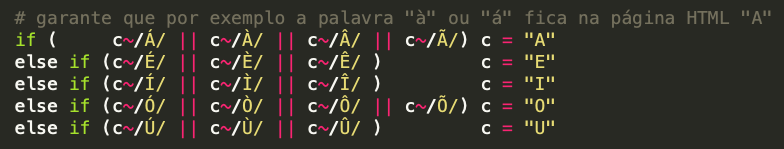
\includegraphics[scale=0.6]{code_fix.png}
	\caption{5 condições para implementar a correção. }
	\label{img:pag}
\end{figure}

Corrigido o problema, finalmente foi implementado o \textbf{formato de apresentação} de cada palavra contida na página do respetivo lema: é apresentada a palavra, seguida da TAG e da \textbf{descrição extensa} da mesma. A seguinte figura mostra a apresentação da página do lema \textbf{"ser"}.

\begin{figure}[H]
	\centering
	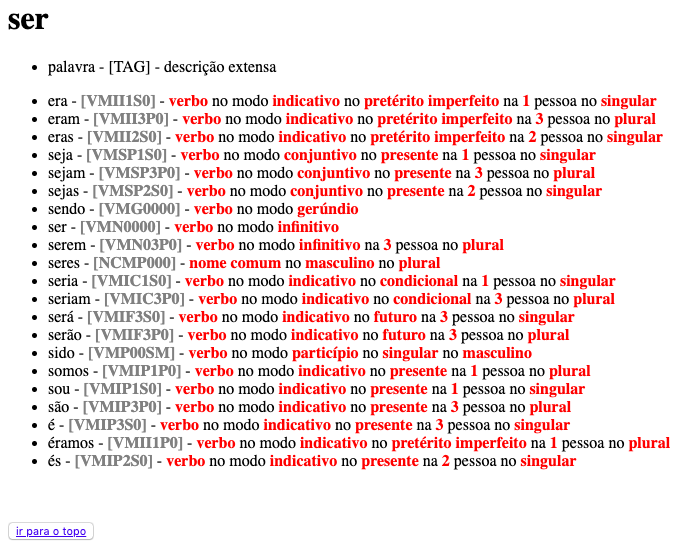
\includegraphics[scale=0.7]{ser.png}
	\caption{página \emph{HTML} do lema \textbf{"ser"}. }
	\label{img:pag}
\end{figure}

Note-se que \textbf{apenas foi implementada a descrição extensa completa de cada TAG para os verbos e nomes}, para os restantes elementos apenas se indica o tipo de elemento, isto é por exemplo para o adjetivo \textbf{"mortal"} apenas se indica que é um adjetivo, em vez de informar completamente, por extenso, que é um adjetivo qualificativo para os dois géneros (masculino e feminino) no singular. A seguinte figura evidencia esta descrição incompleta propositada. 

\begin{figure}[H]
	\centering
	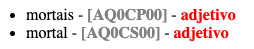
\includegraphics[scale=0.7]{adjetivos.png}}
	\caption{descrição incompleta propositada. }
	\label{img:pag}
\end{figure}

Atente-se que no entanto a \textbf{TAG é sempre apresentada} uma vez que é um requisito obrigatório do problema 4. O motivo de não ter sido desenvolvido a descrição extensa para todos os elementos é que apenas querimos evendicar uma prova de conceito visto que é um extra.


\newpage

\chapter{Utilização, Codificação e Testes dos Scritps}

O grupo definiu uma \emph{Makefile}, que corre os quatro scripts elaborados para cada problema com a utilização do \textbf{awk}. Visto que se trata de scritps processados pelo \emph{gawk}, não foi necessário definir a instalação da aplicação.
\\\\Assim para executar cada problema, basta fazer \emph{make} \textbf{(p1,p2,p3,p4)} para cada respetivo problema, sendo que o ficheiro utilizado como padrão na \emph{Makefile} é o \emph{harrypotter2}, caso se queira proceder ao processamento de outro ficheiro faz-se gawk -f (p1,p2,p3,p4) ficheiroInput.
\\\\Os testes realizados para verficação da resolução de cada problema foram por observações dos resultados em páginas \emph{HTML} e também através de exemplos mais simples gerados pela equipa.

\chapter{Conclusão}
Em suma, os objetivos inicialmente propostos foram cumpridos, dos quais,  a contagem do número de extratos, nomes próprios, listagem dos verbos, substantivos, adjetivos e advérbios e por fim a elaboração do dicionário implicíto no córpora.
\\\\A análise exaustiva dos ficheiros para encontrar os padrões necessários para os campos \emph{FS} e \emph{RS}, foi importante para se conseguir capturar a informação necessária.
\\\\ A nível de trabalho adicional, no problema dois, fez-se a geração do output para uma página \emph{HTML} o problema três, procedeu-se à contagem das ocorrências de cada palavra, ordenando-se as mesmas pelo critério do número de ocorrências, e fez-se o cálculo de alguns dados estatísticos. Por fim, e não menos importante, o problema quatro apresentou o dicionário implícito dos ficheiros fornecidos tal como a lista de palavras derivadas de cada lema, apresentando as mesmas em \emph{HTML} com formato de apresentação equivalente ao dicionário comum.
\emph{HTML}
\appendix % apendice
\chapter{Código do Programa}

Lista-se a seguir o CÓDIGO do API criada pelo grupo:
\begin{verbatim}
function beginHTML(t){
	return "<html><head><meta charset='UTF-8'/></head><body><h1>" t "</h1>"
}


function endHTML(){
	return "</body></html>"
}


function listItem(text){
	return "<li>" text "</li><br>"
}


function link(href, text){
	return "<li><a href=" href ">" text "</a></li>"
}


function createHTMLdir() {
	system("rm -f -r html/")
	system("mkdir html/")
}
\end{verbatim}

\newpage
Lista-se a seguir o CÓDIGO do programa do problema 1:
\begin{verbatim}
#!/usr/local/bin/gawk -f

BEGIN {
	RS = "\n\n"
}

END {
	print "Número de extratos => " NR
}
\end{verbatim}
\newpage
Lista-se a seguir o CÓDIGO do programa do problema 2:
\begin{verbatim}
#!/usr/local/bin/gawk -f

@include "api.awk"

BEGIN {
	RS = "\n"
	FS = " "
}


$4~/NP.*/ {
	counter[$2]++
}


END {
	createHTMLdir()
	print beginHTML("Contador de Ocorrências de Nomes Próprios") > "html/index.html"
	print "<ul>" > "html/index.html"
	
	PROCINFO["sorted_in"] = "comparator"
	for(nome in counter) {
		c = counter[nome]
		print listItem(nome " -> " c) > "html/index.html"
	}

	print "</ul>" > "html/index.html"
	print endHTML() > "html/index.html"
}


function comparator(i1, v1, i2, v2)
{
    if (v1 == v2) return 0;
    else if (v1 > v2) return -1;
    else return 1;
}
\end{verbatim}
\newpage
Lista-se a seguir o CÓDIGO do programa do problema 3:
\begin{verbatim}
#!/usr/local/bin

@include "api.awk"

BEGIN{
	RS = "\n"
	FS = " "
}

$4~/V.*/{	# VERBO
	words["verbos"][tolower($3)]++
}

$4~/N.*/{	# SUBSTANTIVO
	words["substantivos"][tolower($3)]++
}

$4~/A.*/{	# ADJETIVO
	words["adjetivos"][tolower($3)]++
}

$4~/R.*/{	# ADVÉRBIO
	words["adverbios"][tolower($3)]++
}

END{
	createHTMLdir()	# remove e cria a pasta html/	
	listing()
	meta()
	footer()
}

# usado para ordenar o array pelo número de ocorrências de cada palavra
function comparator(i1, v1, i2, v2){
    if (v1 == v2) return 0;
    else if (v1 > v2) return -1;
    else return 1;
}

# lista as palavras de cada tipo em cada ficheiro
function listing(){
	header("Verbos", "verbos.html")
	header("Substantivos", "substantivos.html")
	header("Adjetivos", "adjetivos.html")
	header("Advérbios", "adverbios.html")

	for(tipo in words){
		PROCINFO["sorted_in"] = "comparator"
		for(palavra in words[tipo]){
			if(tipo~"verbos"){
				tiposVerbos++
				verbos = verbos + words[tipo][palavra]
			}
			if(tipo~"substantivos"){
				tiposSubstantivos++
				substantivos = substantivos + words[tipo][palavra]
			}
			if(tipo~"adjetivos"){
				tiposAdjetivos++
				adjetivos = adjetivos + words[tipo][palavra]
			}
			if(tipo~"adverbios"){
				tiposAdverbios++
				adverbios = adverbios + words[tipo][palavra]
			}

			print "<li>" > "html/" tipo ".html"
			print palavra " -----> " words[tipo][palavra] > "html/" tipo ".html"
			print "</li>" > "html/" tipo ".html"
		}
	}
}

# cria e estrutura o index.html
function meta(){
	print beginHTML("Listas") > "html/index.html"
	linkListas()
	estatistica()
}

# faz um header especial para os ficheiros que vão ter as palavras
function header(title, filename){
	print specialbeginHTML("Listas", "index.html", filename1,title) > "html/" filename
	print "<h3 id="filename ">" title " -----> Nº de ocorrências</h2>" > "html/" filename
	print "<ul>" > "html/" filename
}

# finaliza todos os ficheiros
function footer(){
	finally("index.html",0)
	finally("verbos.html",1)
	finally("substantivos.html",1)
	finally("adjetivos.html",1)
	finally("adverbios.html",1)
}

# finaliza um ficheiro
function finally(filename, flag){
	print "</ul>" > "html/" filename
	if(flag == 1)print "<button type="button"><a href=#" filename ">IR PARA O TOPO!!!</a></button><br><br>" > "html/" filename
	print endHTML() > "html/" filename
}

function specialbeginHTML(t1,filename1, filename2, t2){
	return "<html><head><meta charset='UTF-8'/></head><body><h1><a href=" filename1 ">" t1 "</a><a href=" filename2 "> - " t2 "</a></h1>"
}

function estatistica(){
	print "<br><h2>Estatística:</h2>" > "html/index.html"
	print "<ul><h4>" > "html/index.html"
	print "<li>Número de tipos de verbos = " tiposVerbos "</li>"  > "html/index.html"
	print "<li>Número de tipos de substantivos = " tiposSubstantivos "</li>"  > "html/index.html"
	print "<li>Número de tipos de adjetivos = " tiposAdjetivos "</li>"  > "html/index.html"
	print "<li>Número de tipos de advérbios = " tiposAdverbios "</li>"  > "html/index.html"
	print "<li>Total de tipo de palavras = " tiposVerbos + tiposSubstantivos + tiposAdjetivos + tiposAdverbios "</li>"  > "html/index.html"
	print "<br>" > "html/index.html"
	print "<li>Número de ocorrências de verbos = " verbos "</li>"  > "html/index.html"
	print "<li>Número de ocorrências de substantivos = " substantivos "</li>"  > "html/index.html"
	print "<li>Número de ocorrências de adjetivos = " adjetivos "</li>"  > "html/index.html"
	print "<li>Número de ocorrências de advérbios = " adverbios "</li>"  > "html/index.html"
	print "<li>Total de palavras = " verbos + substantivos + adjetivos + adverbios "</li>"  > "html/index.html"

	print "</h4></ul>" > "html/index.html"
}

function linkListas(){
	print "<ul><h3>" > "html/index.html"
	print link("verbos.html", "Verbos") > "html/index.html"
	print link("substantivos.html", "Substantivos") > "html/index.html"
	print link("adjetivos.html", "Adjetivos") > "html/index.html"
	print link("adverbios.html", "Advérbios") > "html/index.html"
	print "</h3></ul>" > "html/index.html"
}
\end{verbatim}

\newpage
Lista-se a seguir o CÓDIGO do programa do problema 4:
\begin{verbatim}
#!/usr/local/bin/gawk -f

@include "api.awk"


BEGIN {
	RS = "\n"
	FS = " "
}

#  VERBO     NOME     ADJETIVO    ADVERBIO   PREPOSIÇÂO  DETERMINANTE  CONJUNÇÂO    PRONOME
$4~/V.*/ || $4~/N.*/ || $4~/A.*/ || $4~/R.*/ || $4~/S.*/ || $4~/D.*/ || $4~/C.*/ || $4~/P.*/ { 	
	
	#      LEMA         WORD       TAG
	dic[tolower($3)][tolower($2)] = $4 
}


END {
	createHTMLdir()
	print beginHTML("DICIONÁRIO") > "html/index.html"

	# percorre a matriz com ordenação alfabética
	PROCINFO["sorted_in"] = "comparator" 

	# imprimir o link no index.html para cada letra 
	# e imprimir o header em cada página {A,B,C, ...}
	for(i=65; i<=90; i++) {
		href = sprintf("_%c_.html", i)
		text = sprintf("%c", i)
		print link(href, text) > "html/index.html"
		print beginHTML(text) > "html/" href

		# para guardar o topo da página
		print "<p id=top></p>" > "html/" href 
	}
	
	for (lema in dic) {
		
		split(lema, str, "")
		c = toupper(str[1]) 

		# garante que por exemplo a palavra "à" ou "á" fica na página HTML "A"
		if (     c~/Á/ || c~/À/ || c~/Â/ || c~/Ã/) c = "A"
		else if (c~/É/ || c~/È/ || c~/Ê/ )         c = "E"
		else if (c~/Í/ || c~/Ì/ || c~/Î/ )         c = "I"
		else if (c~/Ó/ || c~/Ò/ || c~/Ô/ || c~/Õ/) c = "O"
		else if (c~/Ú/ || c~/Ù/ || c~/Û/ )         c = "U"

		# imprime o link para o lema no index.html
		print link(lema ".html", lema) > "html/_" c "_.html" 

		# imprimir a página de cada lema
		printLemaHTML() 
    }
 
    # imprimir o footer em cada página {A,B,C, ...}
    # e imprimir o botão (ir para o topo)
    for(i=65; i<=90; i++) {
		href = sprintf("_%c_.html", i)
		print "<br><br><button type=button><a href=#" top ">ir para o topo</a></button><br><br>" > "html/" href
		print endHTML() > "html/" href
	}

	printEstatistica()
	print endHTML() > "html/index.html"
}


function printEstatistica(){
	print "<br><h2>Estatística:</h2>" > "html/index.html"
	print "<ul><h4>" > "html/index.html"
	print "<li>nº nomes -> " n_nomes "<br></li>" > "html/index.html"
	print "<li>nº adjetivos -> " n_adjetivos "<br></li>" > "html/index.html"
	print "<li>nº adverbios -> " n_adverbios "<br></li>" > "html/index.html"
	print "<li>nº preposicoes -> " n_preposicoes "<br></li>" > "html/index.html"
	print "<li>nº determinantes -> " n_determinantes "<br></li>" > "html/index.html"
	print "<li>nº conjuncoes -> " n_conjuncoes "<br></li>" > "html/index.html"
	print "<li>nº pronomes -> " n_pronomes "<br></li>" > "html/index.html"
	total = n_verbos + n_nomes + n_adjetivos + n_adverbios + n_preposicoes + n_determinantes + n_conjuncoes + n_pronomes
	print "<li>total de palavras -> " total "<br><br></li>" > "html/index.html"
	print "</h4></ul>" > "html/index.html"
}


function printLemaHTML() {
	path = "html/" lema ".html" # caminho para a página do lema
	
	print beginHTML(lema) > path
	print "<ul><li>palavra - [TAG] - descrição extensa</li></ul>" > path

	# para guardar o topo da página
	print "<p id=top></p>" > "html/" href 

	print "<ul>" > path
	for(word in dic[lema]) {
		tag = dic[lema][word]
		split(tag, str, "")
		
		print "<li>" word " - " > path

		# imprimir a TAG
		print "<b style=color:gray;>[" tag "]</b> - " > path	

		if (tag~/V.*/) {
			printVerbo()
			n_verbos++
		}
		else if (tag~/N.*/) {
			printNome() 
			n_nomes++
		}
		else if (tag~/A.*/) {
			printAdjetivo()
			n_adjetivos++
		}
		else if (tag~/R.*/) {
			printAdverbio()
			n_adverbios++
		}
		else if (tag~/S.*/) {
			printPreposicao()
			n_preposicoes++
		}
		else if (tag~/D.*/) {
			printDeterminante()
			n_determinantes++
		}
		else if (tag~/C.*/) {
			printConjuncao()
			n_conjuncoes++
		}
		else if (tag~/P.*/) {
			printPronome()
			n_pronomes++
		}
		print "</li>" > path
	}
	print "</ul>" > path

	# imprime o botão para ir para o TOPO
	print "<br><br><button type=button><a href=#" top ">ir para o topo</a></button><br><br>" > path

	print endHTML() > path
}


function printPronome() {
	print "<b style=color:red;>pronome</b>" > path
}


function printConjuncao() {
	print "<b style=color:red;>conjuncão</b>" > path
}


function printDeterminante() {
	print "<b style=color:red;>determinante</b>" > path
}


function printPreposicao() {
	print "<b style=color:red;>preposição</b>" > path
}


function printAdverbio() {
	print "<b style=color:red;>advérbio</b>" > path
}


function printAdjetivo() {

	# 1 A -> nome
	# -----------------------
	# 2 t -> tipo
	# 3 gen -> género
	# 4 num -> cardinalidade

	print "<b style=color:red;>adjetivo</b>" > path
}


function printNome() {

	# 1 N -> nome
	# -----------------------
	# 2 t -> tipo
	# 3 gen -> género
	# 4 num -> cardinalidade

	print "<b style=color:red;>nome</b>" > path

	t = str[2]; # tipo -> tem sempre
	if (t != "0") {  
		print "<b style=color:red;>" > path
		if (t == "P") print " próprio" > path
		else if (t == "C") print " comum" > path
		else print "___AINDA_SEM_TIPO___" > path
		print "</b>" > path
	}

	printGenero(str[3])
	printCardinalidade(str[4])
}


function printVerbo() {

	# 1 V -> verbo
	# 2 M -> main
	# -----------------------
	# 3 m -> modo
	# 4 t -> tipo
	# 5 p -> pessoa
	# 6 num -> cardinalidade
	# 7 gen -> género	

	print "<b style=color:red;>verbo</b>" > path

	m = str[3] # modo -> tem sempre
	if (m != "0") {
		print " no modo <b style=color:red;>" > path
		if (m == "I") print "indicativo" > path
		else if (m == "S") print "conjuntivo" > path
		else if (m == "G") print "gerúndio" > path
		else if (m == "N") print "infinitivo" > path
		else if (m == "P") print "particípio" > path
		else print "___AINDA_SEM_MODO___" > path
		print "</b>" > path
	}
	
	t = str[4]; # tipo -> pode não não ter (ex: gerúndio ou infinitivo)
	if (t != "0") {  
		print " no <b style=color:red;>" > path
		if (t == "P") print "presente" > path
		else if (t == "S") print "pretérito perfeito" > path
		else if (t == "I") print "pretérito imperfeito" > path
		else if (t == "M") print "pretérito mais que perfeito" > path
		else if (t == "C") print "condicional" > path
		else if (t == "F") print "futuro" > path
		else print "___AINDA_SEM_TEMPO___" > path
		print "</b>" > path
	}
	
	p = str[5] # pessoa -> pode não ter 
	if (p != "0") print " na <b style=color:red;>" p "</b> pessoa" > path
	
	printCardinalidade(str[6])
	printGenero(str[7])
}


function printCardinalidade(num) {

	if (num != "0") {
		print " no <b style=color:red;>" > path
		if (num == "S") print "singular" > path
		else print "plural" > path
		print "</b>" > path
	}
}


function printGenero(gen) {
	if (gen != 0) {
		print " no" > path
		print "<b style=color:red;>" > path
		if (gen == "F") print "feminino" > path
		else print "masculino" > path
		print "</b>" > path
	}
}


function comparator(i1, v1, i2, v2) { # ordena por ordem alfabética

	word1 = i1
	word2 = i2

	if (word1 == word2) return 0;
    else if (word1 > word2) return 1;
    else return -1;
}
\end{verbatim}
\end{document} 
